\section{ Structure et Organisation du Laboratoire}


\subsection{Fonctionnement du Laboratoire}


\subsection{Probléme et Defis du Fonctionnement du Laboratoire}

The Somfy laboratory functions independently of the company's industrial operations. During an in-depth investigation of its operation, a fundamental issue was discovered: the work process is not digital, resulting in a lack of consistency between laboratory test data, test sheets, and test results. This lack of digital integration can cause inefficiencies and gaps in data management, thus affecting the quality and traceability of the tests performed.


\subsection{Intégration du Digital dans les Systèmes de Fonctionnement du Laboratoire}

\begin{figure}[H]
    \centering
    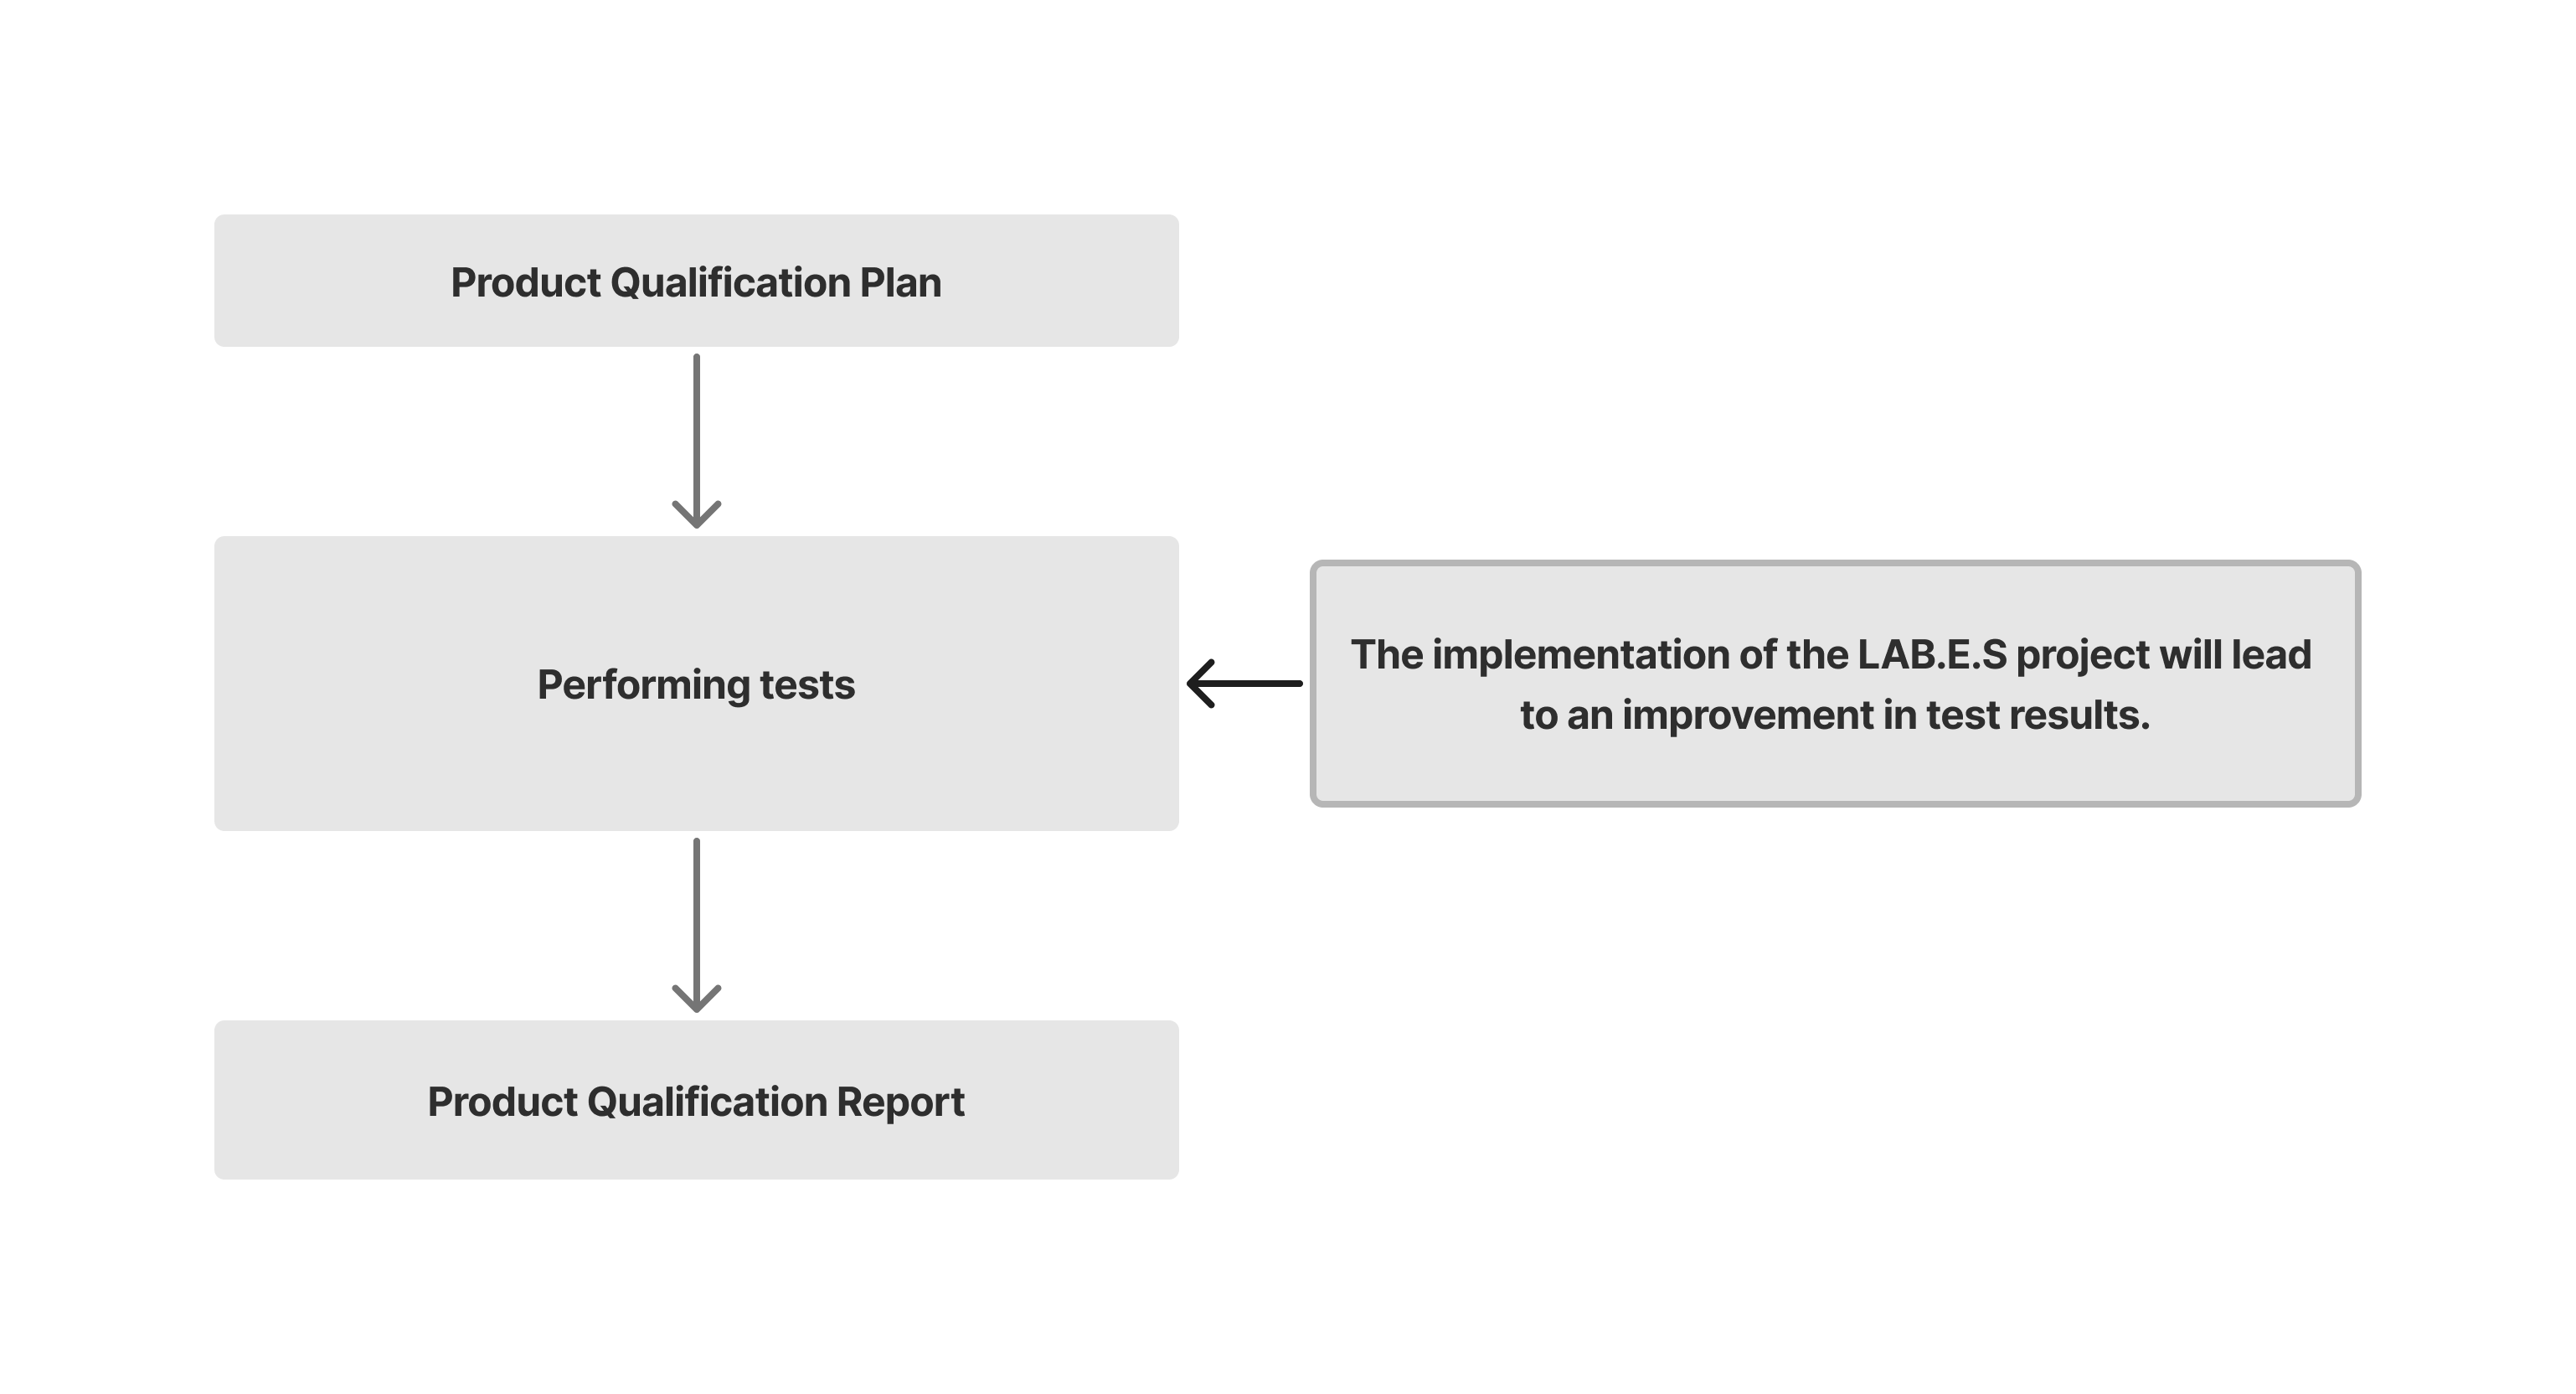
\includegraphics[width=1\textwidth]{chapters/2/img/User Flows (2).png}
    \caption{Somfy Zriba Lab}
    \label{fig:campus}
\end{figure}

\subsection{Exemple d'Application Industrielle existante dans le Site Somfy}

MES is a production planning and supervision tool and these are the key characteristics of SOMFY MES:

\begin{enumerate}
\item Create or edit product data: Oversee the development or revision of production-related documentation, data collecting, and parameter configuration.
\item Schedule: To guarantee effective, real-time production, create and update schedules and manage and optimize the production schedule.

\item Produce: Manage the complete manufacturing process, including start-up, production quantity control, and issue resolution, to guarantee company continuity.
\end{enumerate}
\begin{figure}[H]
    \centering
    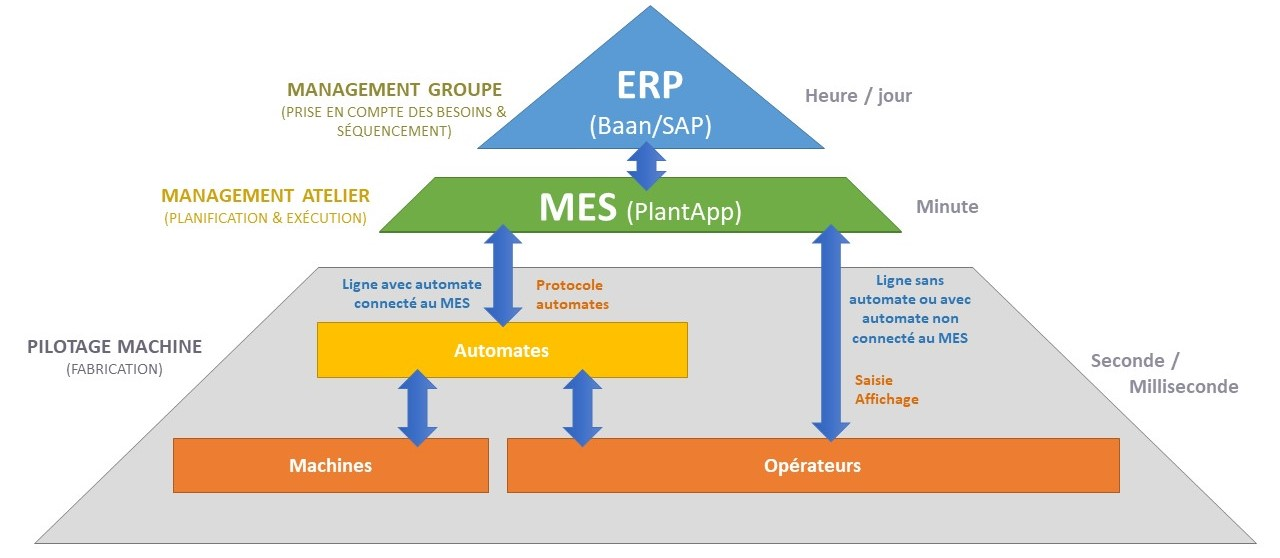
\includegraphics[width=1\textwidth]{chapters/2/img/LES - Molka Abid.jpg}
    \caption{Somfy Zriba Lab}
    \label{fig:campus}
\end{figure}


\subsection{Conclusion de l'Intégration du Digital dans le laboratoire}

The LABES (Laboratory Execution System) application is directly inspired by the MES (Manufacturing Execution System). Just as MES oversees and improves industrial production processes in real time, LABES seeks to convert the laboratory into a completely digitalized and integrated entity.
This development is critical for improving the efficiency, traceability, and quality of laboratory operations, ensuring Somfy's continuing success and increased capacity for innovation.
